\section{Interconnection protocol}
The target interconncection protocol is the UART, which is in charged to allow communication from the FPGA and microcontroller. Main settings regard the baudrate (115200 bit/s), the length of data (8), the parity ODD bit and one stop bit. Considering also the start, the UART peripheral gets busy for 11 cycles.
\newline
\newline
The clock divider generates a train of pulses at 115200 Hz. I talked about clock divider implementation in the previous section. A module called UART synchronizer takes the peripheral busy for 11 cycles. This component receives as input that train of pulses, rather than the FPGA's clock. Conceptually, the synchronizer has a structure very similar to the one of clock divider: a counter, an hardwired register and a comparator. The synchronizer task is to send the shift command to the shift register storing the data to be sent via serial protocol. So, instead of using an equality comparator, I put here an inequality one. Until the value of the counter is less or equal than the value in the hardwired register (10) the UART is being busy. Another difference regards the counter resetting. The UART logic works only in response to an external action, like an interrupt; the train of pulses is generated periodically regardless of buttons status instead. I mean that, after those 11 cycles, the shift command gets disabled but counter is counting up without stopping. A classic counter gets overflow when reaches the all 1s string, turning the peripheral busy in absence of event ($0 \leq 10$). A \textit{saturation counter} keeps at all 1s and has reset to 0 only when an external event has triggered.

\begin{figure}[H]
\centering
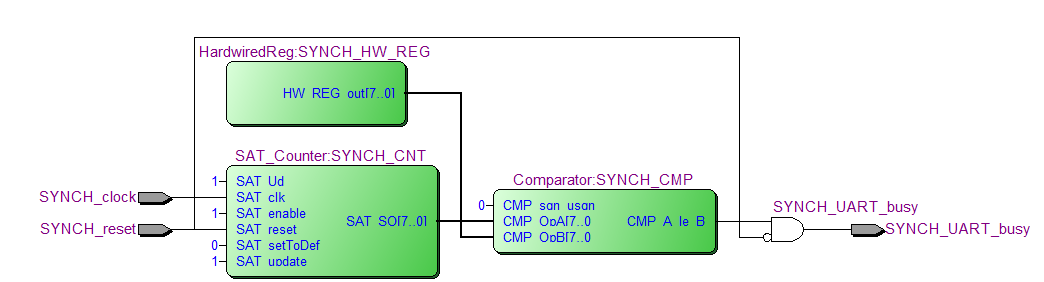
\includegraphics[scale=.8]{Immagini/20}
\label{20}
\caption{UART synchronizer architecture}
\end{figure}